\documentclass[11pt, a4paper, oneside]{report}

% URLs and hyperlinks ---------------------------------------
\usepackage{hyperref}
\hypersetup{
	colorlinks=true,
	linkcolor=blue,
	filecolor=magenta,      
	urlcolor=blue,
}
\usepackage[inline]{enumitem}
\usepackage{xurl}
%---------------------------------------------------


% code snippet -------------------------------------------------------
\usepackage{minted}
% ---------------------------------------------------------------------

% page headers -------------------------------------------------
\usepackage{fancyhdr}
\fancypagestyle{plain}{\fancyhf{}\renewcommand{\headrulewidth}{0pt}}
\pagestyle{fancy}
\fancyhf{}% Clear header/footer
\fancyhead[L]{\nouppercase\leftmark}
\fancyhead[R]{\thepage}
%---------------------------------------------------------------

% adjust a verrrrry big table -------------------------------
\usepackage{adjustbox}
% -----------------------------------------------------------

% titlepage -------------------------------------------------
\usepackage{pdfpages}
%------------------------------------------------------------
% titlepage -------------------------------------------------
\usepackage{svg}
%------------------------------------------------------------
% sudo apt inkscape
% command: pdflatex --shell-escape


% titlepage -------------------------------------------------
\usepackage[font=small,labelfont=bf]{caption}
%------------------------------------------------------------


% multiple figure -------------------------------------------------
\usepackage{graphicx,subcaption} 
%------------------------------------------------------------


% Rn custom item in enumeration -----------------------------
\newcounter{itemadded}
\setcounter{itemadded}{0}


\newcommand{\addeditem}{%
	\addtocounter{enumi}{-1}%
	\stepcounter{itemadded}
	\let\LaTeXStandardLabelEnumi\labelenumi%
	\addtocounter{enumi}{1}
	\renewcommand{\labelenumi}{\arabic{enumi}\lr{R}.}%
	\item 
	% Switch back to old labelling 
	\let\labelenumi\LaTeXStandardLabelEnumi%
}%


\let\LaTeXStandardEnumerateBegin\enumerate
\let\LaTeXStandardEnumerateEnd\endenumerate

\renewenvironment{enumerate}{%
	\LaTeXStandardEnumerateBegin%
	\setcounter{itemadded}{0}
}{%
	\LaTeXStandardEnumerateEnd%
}%
% -----------------------------------------------------------

% tables -------------------------------------------------------
\usepackage{float}
\usepackage{multirow}
\renewcommand{\arraystretch}{1.23}
% ---------------------------------------------------------------------

\usepackage{xepersian}
\settextfont{Yas}
\setdigitfont{Yas}
\setlatintextfont{Yas}

\usepackage{minted}

\begin{document}
	
	\begin{titlepage}
		\centering
		\includesvg[width=4cm]{./layout/besm}\par
	
		\vspace{1cm}
    \includesvg[width=3.2cm]{./layout/logo}\par % Do not include the .svg extension
		
		\vspace{5mm}
		{\LARGE دانشگاه اصفهان}\par
		\vspace{5mm}
		{\Large دانشکده مهندسی کامپیوتر}\par
		
		\vspace{2cm}
		
		{\Large فاز دوم پروژه در مبانی هوش و کاربردها}\par
		\vspace{1cm}
		{\Huge فرآیند تصمیم مارکوف و محیط ناشناخته}\par
		
		
		\vspace{2cm}
		{\Large استاد درس: دکتر حسین کارشناس}\par
		\vspace{0.5cm}
		{\Large دستیار استاد: پوریا صامتی}
		
		\vspace{1.2cm}
		{\Large دانیال شفیعی}\par
		{\Large مهدی مهدیه}\par
		{\Large سید امیررضا نجفی}\par
		
		\vspace{2cm}
		
		% Bottom of the page
		{\large آذر ۱۴۰۳\par}
	\end{titlepage}
	\tableofcontents
	\newpage

	
		\chapter{فرآیند تصمیم مارکوف}
		\section{مقدمه}
	 برای بخش  MDP
	 \footnote{\lr{Markov Decision Process}}
	  در ابتدا تصمیم گرفتیم v\_table  استخراج کنیم که حاوی راه رسیدن به یک خوک هستند. بعد از خوردن هر خوک به v\_table  رفته و طبق سیاست‌هایی که از آن استنتاج کردیم پیش می‌رویم.  این روش مشکلاتی را در پی داشت؛ مثل اینکه ممکن بود یک خوک توسط دیوارها محاصره شده باشد و یا اینکه ممکن بود در مسیر خوردن خوک مورد نظر، بعضی از خوک‌های دیگر نیز به دلیل تصادفی بودن حرکات خورده شوند و مشکلات دیگری که برای حل آنها نیاز به تعداد زیادی شرط بود. این شروط حس را می‌داد که دیگر مسئله را با فرآیند تصمیم مارکوف به صورت عمومی حل نمی‌کنیم و داریم با جزئی نگری زیادی به مسئله نگاه می‌کنیم. این جزئی نگری شاید در بعضی محیط‌ها به نفع ما باشد ولی ممکن است با تغییر محیط برایمان بسیار گران تمام شود.
	 
	 \section{خوشه‌بندی}
	ما تصمیم گرفتیم با استفاده از خوشه‌بندی، خوک‌های موجود در صفحه را به ۲، ۳ یا ۴ خوشه تقسیم  می‌کنیم. سپس با مقایسه، خوشه‌ای که در آن خوک‌ها بهترین نماینده را درون آن خوشه دارند انتخاب کنیم. آنگاه برای هر خوشه یک v\_table می‌سازیم که به خوک‌های موجود در آن خوشه امتیاز مثبت می‌دهیم ولی خوک‌هایی که در آن خوشه نیستند را نادیده می‌گیریم. سپس عامل در هر خوشه  تا جای ممکن خوک‌های موجود را خورده و به سمت خوشه‌ی بعدی حرکت می‌کند و این روند همین‌گونه ادامه پیدا می‌کند تا زمانی که به خوشه‌ی آخر (تخم مرغ) که هدف نهایی است برسیم.
	\subsection{انتخاب تعداد خوشه‌ها}
	سوال کلیدی این است که الگوریتم چگونه متوجه می‌شود به چه ترتیبی v\_table ها را پیمایش کند؟ یا به زبان ساده تر بهتر است ابتدا سیاستهای متعلق به اولین خوشه را اجرا کنیم یا دومین خوشه  را؟
	برای مقایسه، روی تمام مراکز خوشه‌ها جایگشت را حساب می‌کنیم  و بهترین جایگشت را انتخاب می‌کنیم. در بیشترین حالت اگر ۴ خوشه  انتخاب کرده باشیم، $4!$ حالت دارد پس از نظر زمانی نیز لطمه‌ای به الگوریتم نمی‌زند.
	
	\subsection{همگرایی  خوشه‌بندی و تشکیل نقشه‌‌ی گرمایی}
	برای نمونه ما نقشه‌گرمایی محیط راه در خوشه‌بندی به ازای k برابر ۳ در چند تکرار مختلف نمایش می‌دهیم.
	
	\begin{figure}[H]
		\begin{subfigure}{0.40\textwidth}
			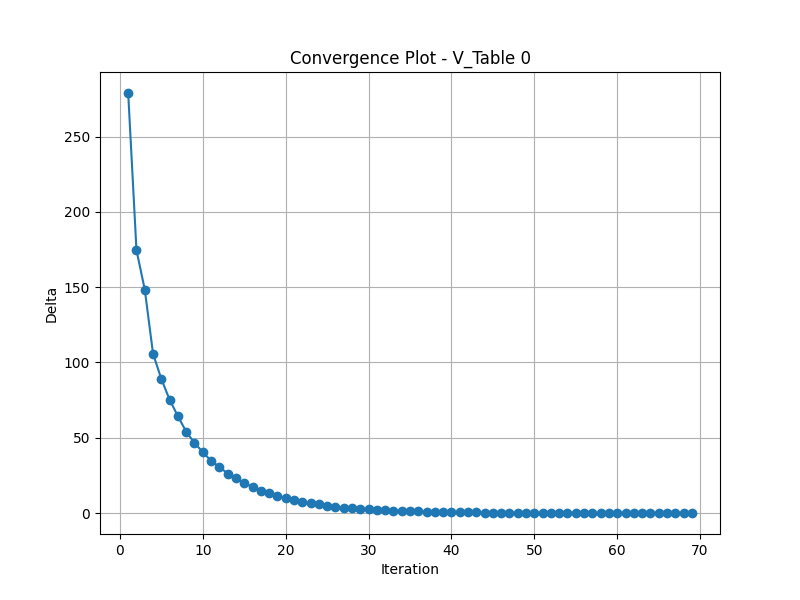
\includegraphics[width=\textwidth]{./images/conv}
			\caption{همگرایی خوشه‌بندی}
			\label{fig:i}
		\end{subfigure}
		\hfill
		\begin{subfigure}{0.40\textwidth}
			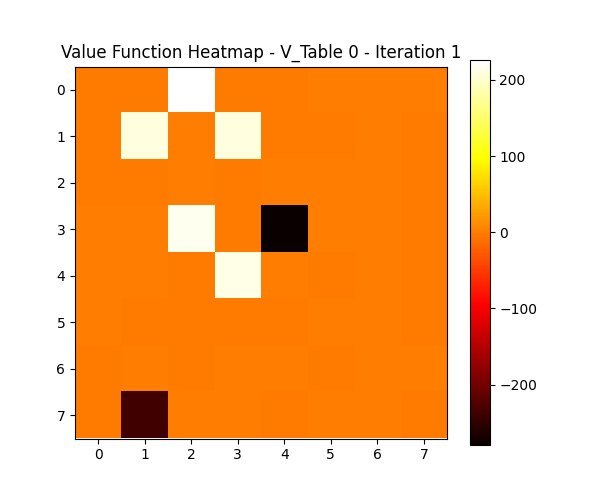
\includegraphics[width=\textwidth]{./images/iter1}
			\caption{تکرار اول}
			\label{fig:j}
		\end{subfigure}
		
		\medskip
		\begin{subfigure}{0.40\textwidth}
			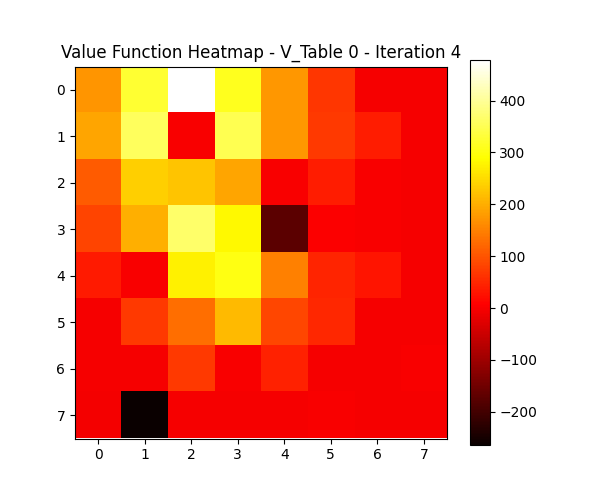
\includegraphics[width=\textwidth]{./images/iter4}
			\caption{تکرار چهارم}
			\label{fig:k}
		\end{subfigure}
		\hfill
		\begin{subfigure}{0.40\textwidth}
			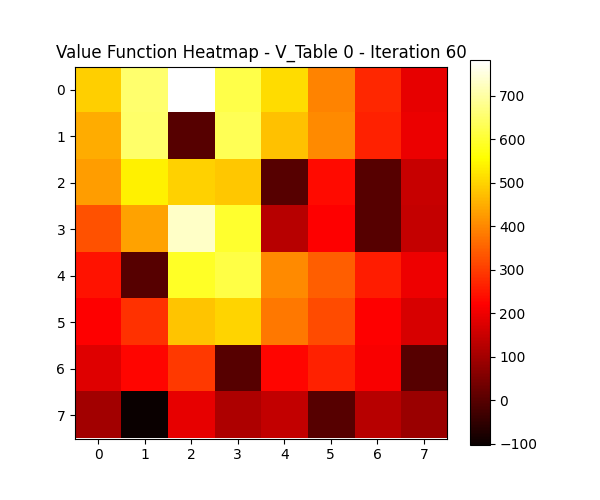
\includegraphics[width=\textwidth]{./images/iter60}
			\caption{تکرار شصتم}
			\label{fig:l}
		\end{subfigure}
		
		\caption{نمونه‌ای از همگرایی خوشه‌بندی به ازای k برابر ۳ }
		\label{Clustering}
		
	\end{figure}
	
	
	
	
	
\section{خروجی الگوریتم}
در ادامه خروجی از تحلیل الگوریتم روی یک نمونه از محیط را می‌بینیم.





 \begin{LTR}
	\begin{minted}[frame=lines, fontsize=\small, tabsize=4, texcomments=false,
		breaklines=true, breakanywhere=true]{text}
Best clustering with 4 clusters:
Cluster 1: [(5, 1), (5, 3), (6, 2)], Centroid: 33.5, 0.2
Cluster 2: [(0, 1), (0, 3)], Centroid: 0.0, 0.2
Cluster 3: [(6, 6)], Centroid: 0.6, 0.6
Cluster 4: [(0, 6), (0, 7)], Centroid: 0.0, 5.6
	\end{minted}
\end{LTR}

\begin{figure}[H]
	\begin{subfigure}{0.40\textwidth}
		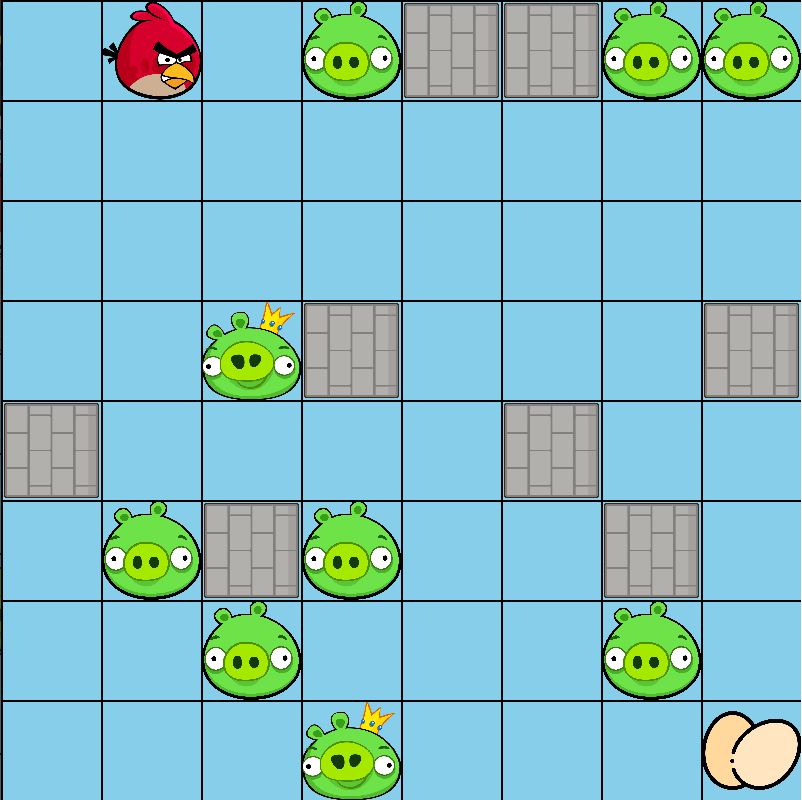
\includegraphics[width=\textwidth]{./images/mdp1}
		\caption{شروع}
		\label{fig:a}
	\end{subfigure}
	\hfill
	\begin{subfigure}{0.40\textwidth}
		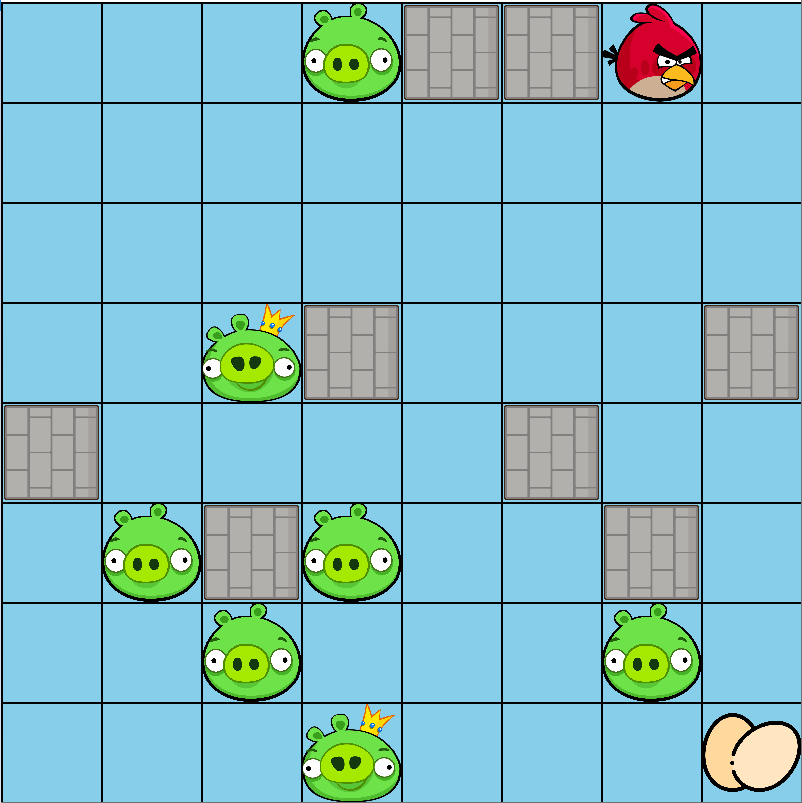
\includegraphics[width=\textwidth]{./images/mdp2}
		\caption{حرکت به سمت خوشه‌ی اول}
		\label{fig:b}
	\end{subfigure}
	
	\medskip
	\begin{subfigure}{0.40\textwidth}
		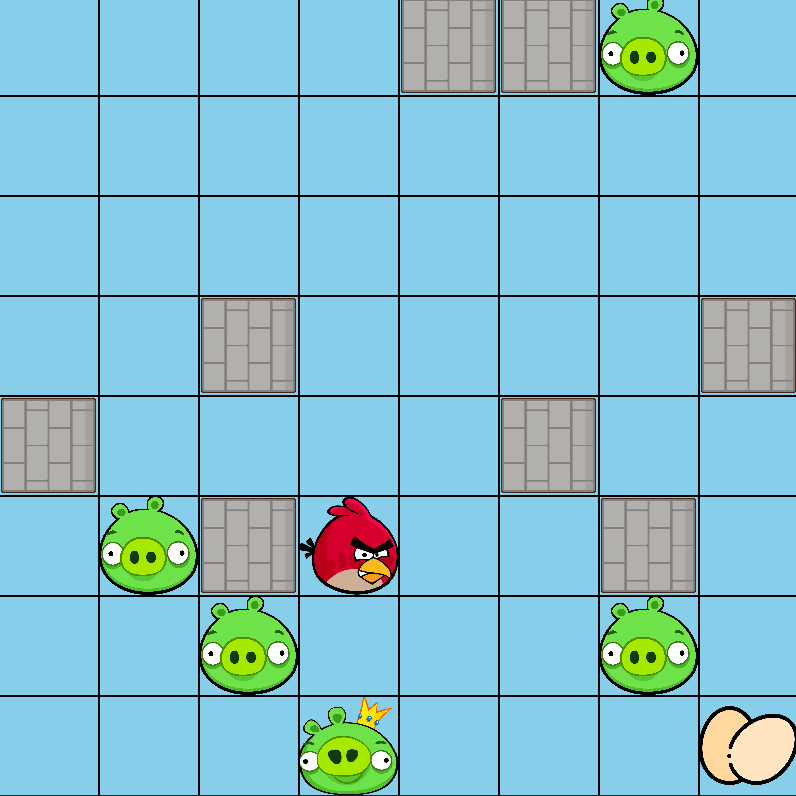
\includegraphics[width=\textwidth]{./images/mdp3}
		\caption{حرکت به سمت خوشه‌ی دوم}
		\label{fig:c}
	\end{subfigure}
	\hfill
	\begin{subfigure}{0.40\textwidth}
		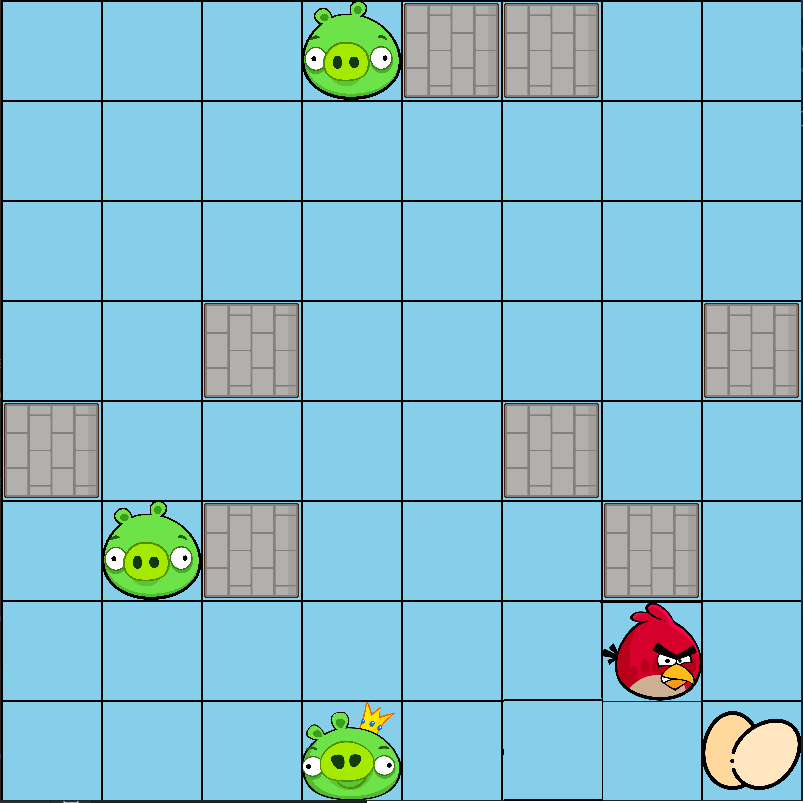
\includegraphics[width=\textwidth]{./images/mdp4}
		\caption{حرکت به سمت  خوشه‌ی سوم (تخم‌مرغ)}
		\label{fig:d}
	\end{subfigure}
	
	\caption{روند حرکت پرنده‌ی خشمگین درون یک محیط تصادفی نمونه }
	\label{MDP}
	
\end{figure}


	
		
		
		
		
		
	\chapter{محیط ناشناخته}
	\section{مقدمه}
	در این بخش از پروژه ما قصد داشتیم با تعداد محدودی تکرار و گردش \footnote{Explore} در محیط ناشناخته
	\footnote{Unknown Environment}
	به یک قاعده برسیم که در آن بتوانیم با استفاده از، به نحوی در این محیط تصادفی پرنده را هدایت کنیم که بیشترین امتیاز ممکن را کسب کند. نکات قابل توجه در این پروژه این است که نباید به TNT برخورد کنیم و تعداد حرکات هم محدود است و نمی‌توانیم بی‌نهایت در محیط بگردیم تا همه‌ی حالت‌ها را بدست بیاوریم.
	
	\section{شیوه‌ی پیاده‌سازی الگوریتم QLearning}
	در مرحله‌ی اول ما یک ماتریس ۸ در ۸ در ۴ داشتیم که امتیاز هر کنش در هر حالت را مشخص می‌کرد. حالت‌ها نمایان‌گر نقطه‌ی که پرنده در آن وجود داشت بودند.
	\subsection{ابرپارامترهای آموزش}
	برای تغییرات 
	  \href{https://www.geeksforgeeks.org/q-learning-in-python/}{مقادیر جدول Q} 
	  یک سری ابر پارامتر وجود دارد.  $\gamma$ در کد ما تحت عنوان فاکتور تخفیف معرفی شده است و $\alpha$  تحت عنوان سرعت آموزش.
	\begin{equation}
		Q(s_t, a_t) \leftarrow Q(s_t, a_t) + \alpha \left[ r_{t+1} + \gamma \max_{a} Q(s_{t+1}, a) - Q(s_t, a_t) \right]
	\end{equation}
	در هر اپیزود از اجرای الگوریتم، حالت به عنوان ورودی داده می‌شود و سپس بهترین کنش از جدول انتخاب می‌شود. سپس با انجام کنش به کمک تابع step می‌دهیم و خروجی آن را دریافت می‌کنیم و توابع و حالات جدید را بدست می‌آوریم.
	 

	 	
	 	\subsection{همگرایی مقادیر}
	برای اینکه بعد از مدتی همگرا شود، ما از تکنیک
\href{https://www.geeksforgeeks.org/epsilon-greedy-algorithm-in-reinforcement-learning/}{\lr{Epsilon Greedy} }
استفاده کردیم. در این راهبرد. در اوایل اجرا، پرنده تا جای ممکن تصادفی عمل می‌کند. اما به مرور زمان با توجه به نتایج به دست آمده بهترین کنش را انتخاب می‌کند. نرخ کاهش نیز بدین صورت است که تا زمانی که نتیجه در هر حال بهتر شدن است، همچنان اپسیلون و نرخ یادگیری تغییری نمی‌کند اما به محض کاهش پاداش کل برای اپسیلون گریدی و افزایش value\_diff برای سرعت یادگیری، مقادیر کاهش پیدا می‌کنند.
\begin{center}
	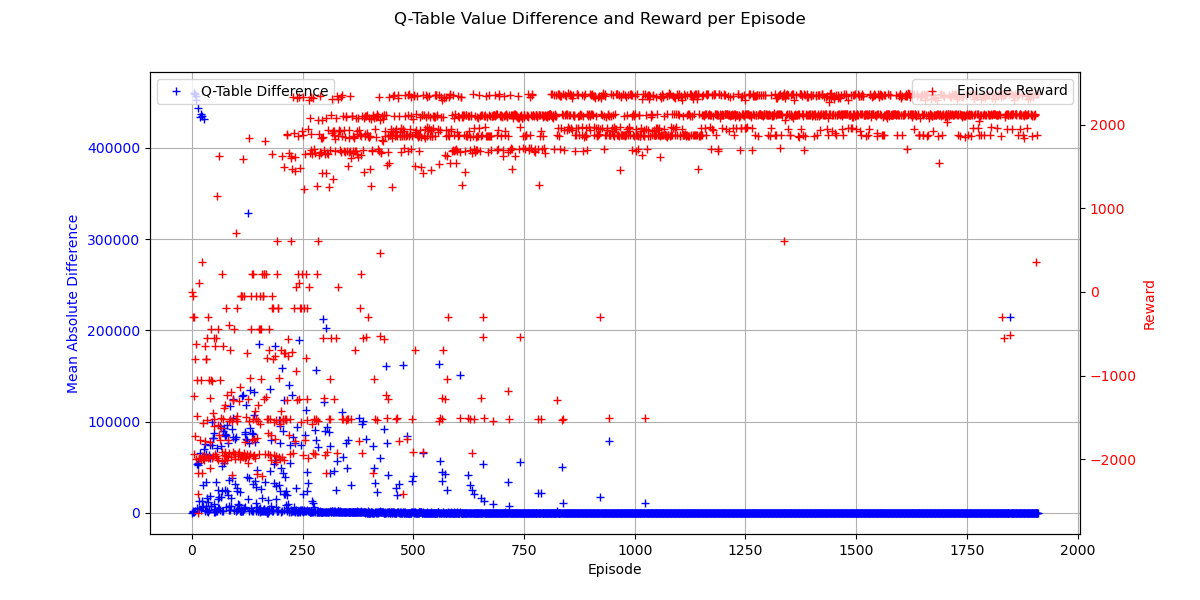
\includegraphics[width=12cm]{./images/value_diff.png}
	\captionof{figure}
	{همگرایی value\_diff در یک محیط نمونه که پس از ۱۰ بار کوچک‌تر شدن اپسیلون از ۱۰ الگوریتم متوقف شده است.}
\end{center}
	
	\subsection{استخراج سیاست}
	در ابتدای کار وقتی شرایط زنده بودن خوک‌ها را در نظر نگرفته بودیم، می‌توانستیم یک سیاست واحد استخراج کنیم اما بعد از آن، ما از بین اکشن‌ها مُد می‌گیریم تا یک حس از اینکه در هر حالت به چه سمتی حرکت می‌کند مشخص شود. برای خانه‌هایی که مقادیرشان مشخص نیست، الگوریتم به صورت تصادفی سیاست استخراج می‌کند.
	

	\begin{center}
\begin{figure}[H]
	\begin{subfigure}{5cm}
		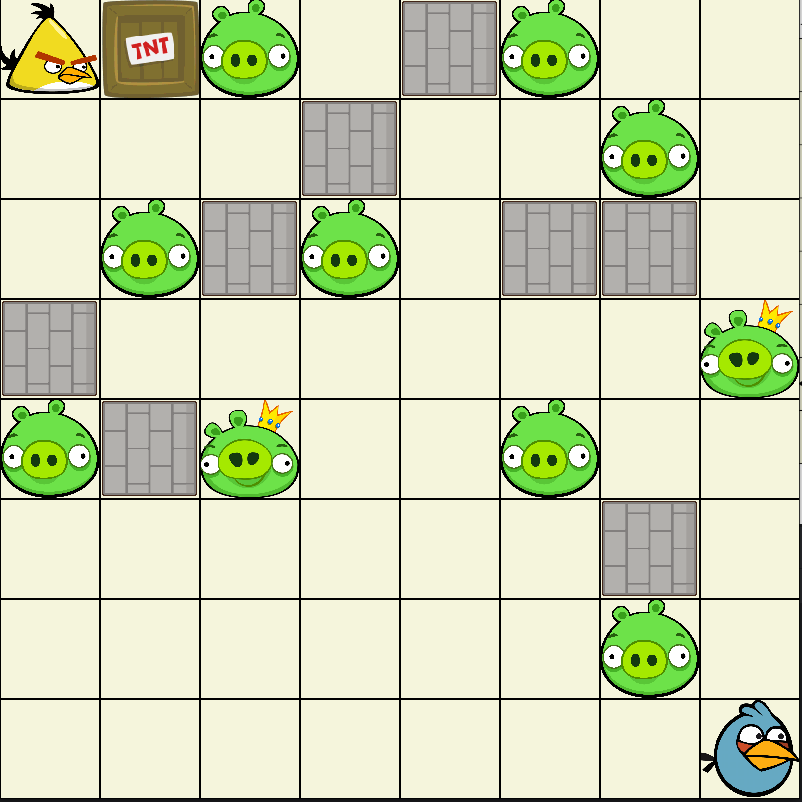
\includegraphics[width=5cm]{./images/env1.png}
		\caption{محیط نمونه}
		\label{fig:e}
	\end{subfigure}
	\hfill
	\begin{subfigure}{5cm}
		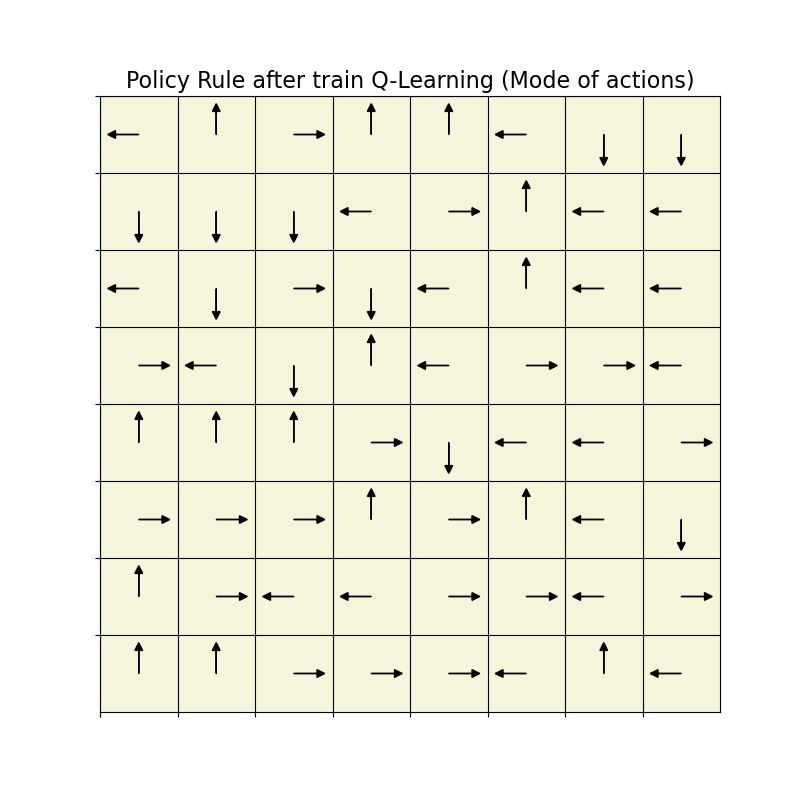
\includegraphics[width=5cm]{./images/policy.png}
		\caption{مد کنش‌ در حالت‌ها در محیط متناظر}
		\label{fig:f}
	\end{subfigure}
	
	\caption{ استخراج سیاست به شیوه‌ی مد گرفتن از کنش‌ها در هر حالت }
	\label{Policy}
	
\end{figure}
	\end{center}
	
	\subsection{سایر ویژگی‌ها}
	\paragraph{مهندسی پاداش}
	وقتی الگوریتم به پایان می‌رسد، یک پاداش ۱۰۰۰- داریم که اگر این پاداش روی یک حالت و کنش برود، حتی اگر آن کنش خوب باشد، باعث می‌شود دیگر سمت این کنش نرویم! ما باید این اثر را حذف کنیم.
	همچنین چنین در نظر گرفته بودیم که اگر یک حالت و کنشی در یک اپیزود دفعات متکرر اجرا شد، به آن امتیاز منفی بدهیم که البته این باعث همگرایی نمی‌شود و ممکن است نتابج بدتری بدهد. همچنین برای اینکه از ملکه‌ها رد شویم و در دام آن‌ها نیفتیم، فرض کردیم اگر از آن‌ها بگذریم، امتیاز منفی کمتری دارد که البته این هم حالب نبود. در نهایت هم مقادیر جدول Q را به ازای همه‌ی کنش‌های آن حالت بروز می‌کردیم تا هیچ کنشی حتی کنش مقداردهی نشده هم به سمت TNT نرود.
	
		\paragraph{مصورسازی}
	برای نمایش اینکه در هر حالت چه کنشی بیشتر موردتوجه است و چه کنشی مضر است، از یک نقشه گرمایی استفاده کردیم که جهت‌های ممکن را به ما نشان می‌دهد. به این منظور کنش‌های هر حالت نرمالایز می‌شود و بر اسا مقادیر ۰ تا یک رنگ پیدا می‌کند. خانه‌هایی که همه‌ی آن‌ها قرمز هستند یعنی هیچ‌گاه مقداردهی نشده‌اند و خانه‌هایی که هر سه خانه سبز هستند یعنی یکی از خانه‌ها مقدار منفی دارد و احتمالا قدر مطلق آن بسیار زیاد است. واضح است خانه‌ای که TNT در آن موجود است از هر ۴ جهت قرمز شده است.
		\begin{center}
		\begin{figure}[H]
			\begin{subfigure}{5cm}
				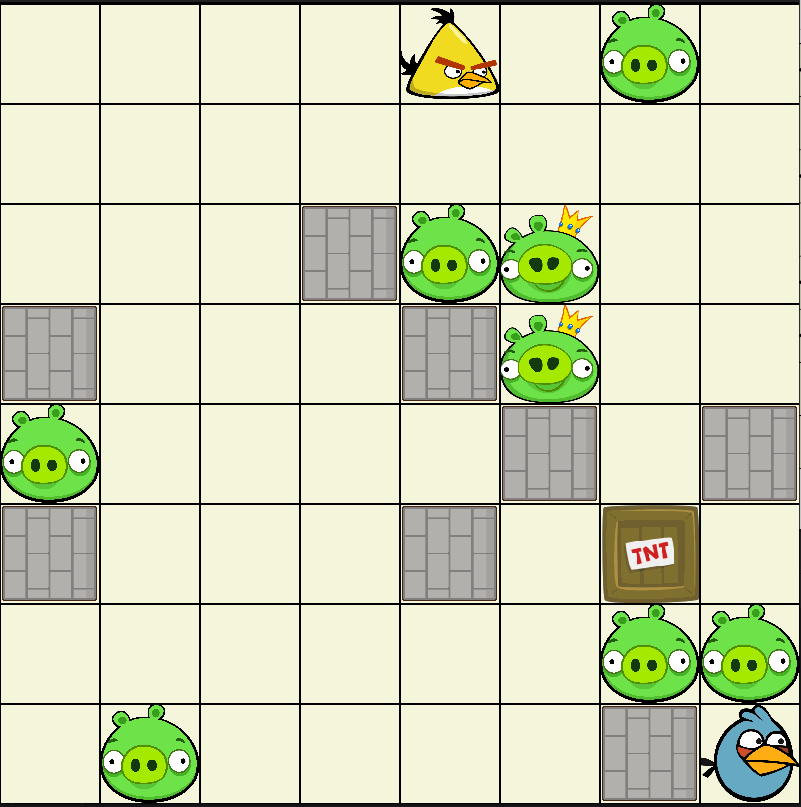
\includegraphics[width=5cm]{./images/env2.png}
				\caption{محیط نمونه}
				\label{fig:g}
			\end{subfigure}
			\hfill
			\begin{subfigure}{5cm}
				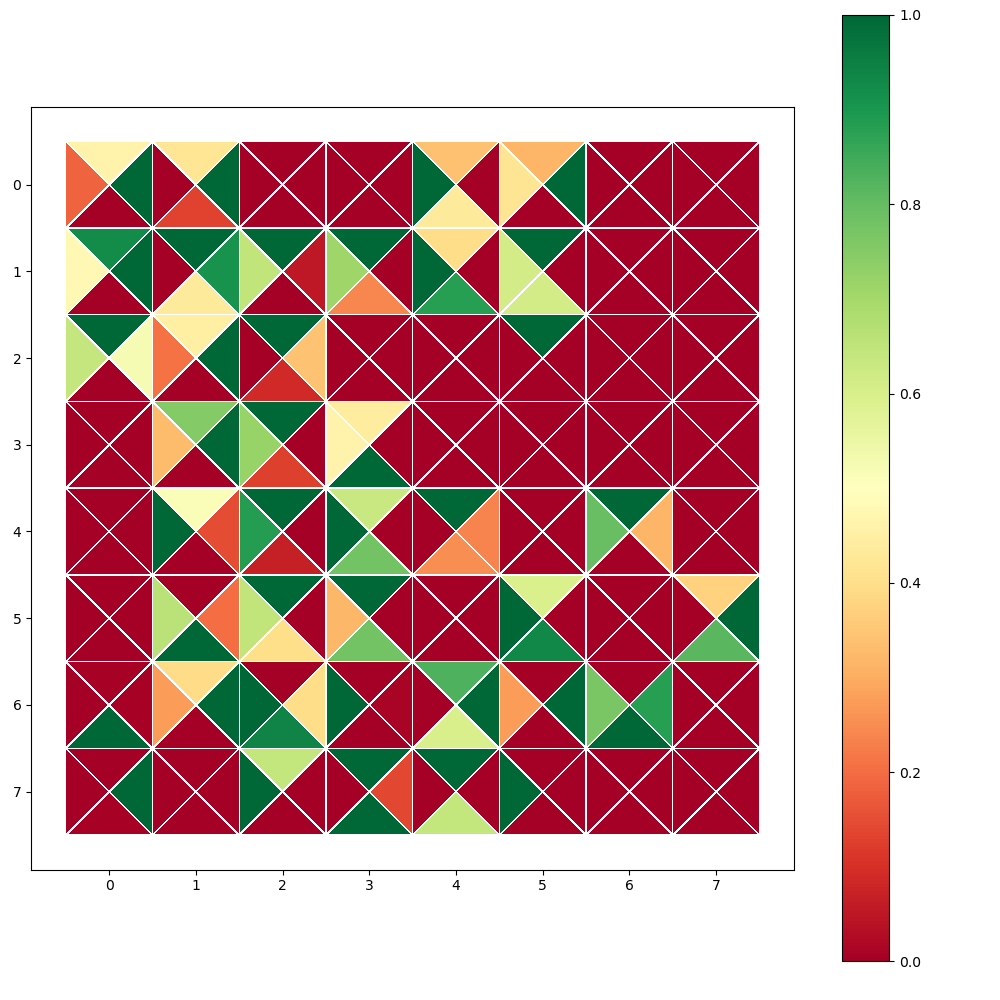
\includegraphics[width=5cm]{./images/htmp.png}
				\caption{نمونه نقشه گرمایی در حالی که هیچ‌کدام از خوک‌ها خورده نشده‌اند}
				\label{fig:h}
			\end{subfigure}
			
			\caption{نقشه گرمایی جهت حرکت بر اساس جدول Q}
			\label{Heatmap}
			
		\end{figure}
	\end{center}
	
	\paragraph{اثرپذیری از حالت خوک‌ها}
	به کمک این ویژگی متناسب با اینکه هر خوکی خورده شده است یا نه یک جدول سیاست کنش داریم. یعنی به‌جای ۱ جدول، ۲۵۶ جدول داریم که البته بسیاری از آن‌ها هرگز مقداردهی نمی‌شوند ولی همین‌هایی که پر می‌شوند به ما کمک می‌کنند تا امتیاز بسیار بالایی کسب کنیم و به‌خاطر یک خوک خورده شده گرفتار حلقه نشویم و محدودیت حرکتی نخوریم.
	
	\section{خروجی}
	نمونه‌ی خروجی این الگوریتم برای محیط نسبتا سختی که در شکل
	  \ref{fig:g}
	نمایش داده شده است به نحو زیر می‌باشد:
	 \begin{LTR}
		\begin{minted}[frame=lines, fontsize=\small, tabsize=4, texcomments=false,
			breaklines=true, breakanywhere=true]{text}
[False, False, False, False, False, False, False, False]
Episode finished with reward: 2347
[False, False, False, False, False, False, False, False]
Episode finished with reward: 2336
[False, False, False, False, False, False, False, False]
Episode finished with reward: 2285
[False, False, False, False, False, False, False, False]
Episode finished with reward: 2329
[False, False, False, False, False, False, False, False]
Episode finished with reward: 2303
MEAN REWARD: 0.2320
		\end{minted}
	\end{LTR}
	در هر ۵ حالت همه‌ی خوک‌ها خورده شده‌اند و امتیاز بالایی کسب شده است.
	
	
	\section{شبکه‌ی عصبی}
	\subsection{مقدمه}
	Q-Learning عمیق 
	یا شبکه‌ی Q عمیق
	\footnote{\lr{\href{https://medium.com/@samina.amin/deep-q-learning-dqn-71c109586bae}{Deep Q Network}}}
	 همان توسعه یافته‌ی الگوریتم Q-Learning است که در آن از شبکه‌های عصبی برای یادگیری عمیق و تقریب Q استفاده می‌شود.
	   Q-Learning
	    سنتی برای محیط‌هایی با تعداد حالت‌های کم و محدود به خوبی کار می‌کند، اما به دلیل اندازه جدول Q با فضاهای حالت بزرگ یا پیوسته مشکل دارد.
	      Q-Learning
	  عمیق    با جایگزین کردن جدول Q با یک شبکه عصبی که می تواند مقادیر Q را برای هر جفت حالت-عمل تقریبی بزند و بر این محدودیت غلبه کند.
	
	\subsection{پیاده‌سازی}
	\paragraph{ساختار شبکه}
	\textbf{لایه اول:} 
	ورودی با اندازه ۶۴ (که نشان‌دهنده‌ی وضعیت محیط ۸ در ۸ است) به ۱۲۸ نورون متصل می‌شود.
\textbf{لایه دوم:} 
 ۱۲۸ نورون به ۶۴ نورون متصل می‌شود.
\textbf{لایه خروجی:}  ۶۴ نورون به تعداد کنش‌های ممکن ( بالا، پایین، چپ، راست) متصل می‌شود.
\textbf{ تابع فعال‌سازی:}  از تابع ReLU برای افزودن غیرخطی بودن به شبکه استفاده می‌شود.
	
\paragraph{اپیزودها}
ما یک بهنیه‌ساز و تابع خطا تعریف می‌شود. همچنین وضعیت محیط به بردار ۸ در ۸ تبدیل می‌شود. که این بردار ورودی شبکه عصبی است.
	هر سلول بر اساس پاداش خود آن مقدار خاصی به بردار اضافه می‌کند.
سپس یک کنش انتخاب می‌شود و یک قدم برداشته می‌شود. بعد با استفاده از راهبر اپسیلون گریدی یک اقدام تصادفی یا اقدامی با بیشترین مقدار انتخاب می‌شود.
سپس مدل بر اساس پاداش تجربیات خود را ذخیره می‌کند و وزن‌های شبکه‌ی  عصبی بروزرسانی می‌شود.
	
	 سیاست نهایی با انتخاب اقدام با بیشترین مقدار Q برای هر وضعیت ممکن استخراج می‌شود.
	

	
	
\end{document}